\documentclass[a4paper,8pt]{article}

\usepackage[T1]{fontenc}
\usepackage[swedish]{babel}
\usepackage[utf8]{inputenc}

\usepackage{lmodern}
\usepackage{amsmath}
\usepackage{graphicx}
\usepackage{amsfonts}

% Tikz
\usepackage{tikz}
\usetikzlibrary{shapes,arrows,positioning,topaths}
\tikzstyle{block} = [rectangle, draw, 
    text width=5em, text centered, rounded corners, minimum height=4em]
\tikzstyle{line} = [draw, -latex']


\usepackage{bytefield}
\title{\huge{D2K2} \vspace{1cm}\\ 
  \large{TSEA43 - Kravspec}}
\author{Johan Angelstam, Caj Larsson, Erik Lindholm}
\date{2012-01-18}

\begin{document}

\maketitle
\vfill
\begin{tabular}{ l l l }
  Version & Datum & \\
  1.0     & 2012-01-18 & Första versionen \\
\end{tabular}

\thispagestyle{empty}

\pagebreak

\section{Beskrivning}
Vi vill bygga ett digitalur med knapp för att ställa tiden, en
knapp för att växla till att se och kunna sätta en
alarmtid och en reset-knapp. Konstruktionen kommer bestå av en CPLD,
tre studsfria knappar och en åttateckens-alfanumeriskdisplay.

\section{Blockschema}
\begin{figure}[h]
\centering
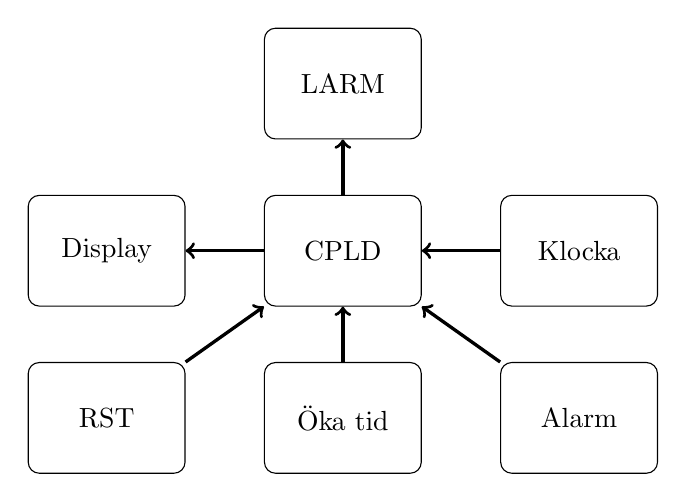
\begin{tikzpicture}[node distance = 3 cm, auto]
  \node [block] (larm) {LARM};
  
  \node [block, below= 2em of larm] (cpld) {CPLD};
  \node [block, left of= cpld] (display) {Display};
  \node [block, right of= cpld] (klocka) {Klocka};

  \node [block, below= 2em of cpld] (oka) {Öka tid};
  \node [block, left of= oka] (rst) {RST};
  \node [block, right of= oka] (alarm) {Alarm};
  
  \draw [->, very thick] (cpld) to (larm);
  \draw [->, very thick] (cpld) to (display);
  \draw [->, very thick] (klocka) to (cpld);
  \draw [->, very thick] (rst) to (cpld);
  \draw [->, very thick] (oka) to (cpld);
  \draw [->, very thick] (alarm) to (cpld);
\end{tikzpicture}
\end{figure}

\section{Krav}
För att inte sätta ribban för högt har vi varit tämligen restriktiva med våra
 ska-krav.

\subsection{Ska}
\begin{enumerate}
  \item Konstruktion på högst en CPLD.
  \item Alarmfunktion.
  \item Möjlighet att sätta tiden. 
  \item Reset-knapp.
\end{enumerate}

\end{document}
